% Use only LaTeX2e, calling the article.cls class and 12-point type.

\documentclass[12pt]{article}

% Users of the {thebibliography} environment or BibTeX should use the
% scicite.sty package, downloadable from *Science* at
% www.sciencemag.org/about/authors/prep/TeX_help/ .
% This package should properly format in-text
% reference calls and reference-list numbers.

\usepackage{scicite}

% Use times if you have the font installed; otherwise, comment out the
% following line.

\usepackage{times}
\usepackage{graphicx}
\usepackage{caption}
\usepackage{subcaption}
\usepackage{stfloats}
% The preamble here sets up a lot of new/revised commands and
% environments.  It's annoying, but please do *not* try to strip these
% out into a separate .sty file (which could lead to the loss of some
% information when we convert the file to other formats).  Instead, keep
% them in the preamble of your main LaTeX source file.


% The following parameters seem to provide a reasonable page setup.

\topmargin 0.0cm
\oddsidemargin 0.2cm
\textwidth 16cm 
\textheight 21cm
\footskip 1.0cm


%The next command sets up an environment for the abstract to your paper.

\newenvironment{sciabstract}{%
\begin{quote} \bf}
{\end{quote}}


% If your reference list includes text notes as well as references,
% include the following line; otherwise, comment it out.

\renewcommand\refname{References and Notes}

% The following lines set up an environment for the last note in the
% reference list, which commonly includes acknowledgments of funding,
% help, etc.  It's intended for users of BibTeX or the {thebibliography}
% environment.  Users who are hand-coding their references at the end
% using a list environment such as {enumerate} can simply add another
% item at the end, and it will be numbered automatically.

\newcounter{lastnote}
\newenvironment{scilastnote}{%
\setcounter{lastnote}{\value{enumiv}}%
\addtocounter{lastnote}{+1}%
\begin{list}%
{\arabic{lastnote}.}
{\setlength{\leftmargin}{.22in}}
{\setlength{\labelsep}{.5em}}}
{\end{list}}


% Include your paper's title here

\vspace{-3cm}

\title{Predicting Cancer Regulatory Networks: A Variational Bayesian Approach} 


% Place the author information here.  Please hand-code the contact
% information and notecalls; do *not* use \footnote commands.  Let the
% author contact information appear immediately below the author names
% as shown.  We would also prefer that you don't change the type-size
% settings shown here.

\author
{Kevin Tee, Michael Liang \\
\\
\normalsize{Department of Computer Science}\\
\normalsize{University of California, Berkeley}\\
\\
\normalsize\texttt{\{kevintee,liangmichael\}@berkeley.edu} 
}

% Include the date command, but leave its argument blank.

\date{}



%%%%%%%%%%%%%%%%% END OF PREAMBLE %%%%%%%%%%%%%%%%



\begin{document} 

% Double-space the manuscript.

\baselineskip24pt
\setlength{\parskip}{1em}
\setlength{\parindent}{0em}
% Make the title.

\maketitle 



% Place your abstract within the special {sciabstract} environment.

\begin{sciabstract}
For many human diseases, such as cancer, gene regulatory networks can provide insight into disease etiology and pathogenesis. Recent technological advances in the measurement of genome-wide gene expression allow for many computational inferences of such networks. In this method, we use a Bayesian approach to constructing these networks, comparing our results to MERLIN. Both methods were applied to publicly available breast tumor microarray data from the TCGA database. Additionally, we validate our results with comparison to ChIP-seq data and Gene Ontology analysis, suggesting advantages and disadvantages to our method. 

%For many human diseases, such as cancer, gene regulatory networks can provide insight into disease etiology and pathogenesis. Recent technological advances in the measurement of genome-wide gene expression allow for many computational inferences of such networks. The high dimensionality of gene expression data and insufficient sample measures often resulted in the predicted regulatory relations that were not supported by biological evidence. The lack of consensus among these inference methods is another concern. Thus, validation of these inferred networks became crucial. To that end, we compared the inferred gene regulatory networks (GRN) from MERLIN and ???. Both methods were applied to publicly available breast tumor microarray data from the TCGA database. We found [summarize similarities and differences: overall gene regulatory network visualization is similar; \% consensus and \% disagreement in terms edges and clustering?]. Based on Gene Oncology analysis, approximately \% of regulatory relations inferred by MERLIN and \% by ??? showed evidence of biological relevance. The minor (or remarkable) differences in the GRN inferred by these two methods pointed to the possible validation approach through comparisons of multiple inference methods and Gene Oncology analysis.
\end{sciabstract}

% In setting up this template for *Science* papers, we've used both
% the \section* command and the \paragraph* command for topical
% divisions.  Which you use will of course depend on the type of paper
% you're writing.  Review Articles tend to have displayed headings, for
% which \section* is more appropriate; Research Articles, when they have
% formal topical divisions at all, tend to signal them with bold text
% that runs into the paragraph, for which \paragraph* is the right
% choice.  Either way, use the asterisk (*) modifier, as shown, to
% suppress numbering.

\section*{Introduction}
Cancer is a disease of the genome that is associated with accumulation of mutational events that lead to disregulation of the cellular system. Genes involved in cancer development and progression are classified as oncogenes, tumor suppressor genes and genomic stability genes [1]. These genes have a key role in the regulation of the cell-cycle, proliferation and cell differentiation, and in the regulation of apoptosis [2]. Mutations in over 100 genes are known to drive tumorgenesis, affecting a broad classes of proteins such as transcription factors, chromatin remodelers, growth factors (e.g.,EGFR), growth factor receptors (e.g.,HER2), signal transducers, regulators of apoptosis and DNA repair genes [2]. Within any given tumor there are between 2-8 mutated �driver genes� modulating the activity of critical molecular pathways [3]. Pilot studies by TCGA and others demonstrated that patients harbor genomic alterations or aberrant expression in different genes and these genes often participate in a common pathway [4,5], indicating that pathway-level genomic perturbations are key features in the underlying cancer biology. Gene regulatory network (GRN) in these cancer pathways has been recognized as potentially important prognosis markers in risk of metastasis or ultimately the target for personalized treatments [6].

High-throughput technologies have produced enormous amount of genome-wide gene expression data. Many data driven mathematical and computational approaches have been developed for probing the molecular interactions of cancer pathways. The molecular interactions between the genes and their products are complex and dynamic. Due to the high dimensionality of gene expression data and insufficient sample measures, the GRN with high prediction accuracy may not reveal the true biological relations. Further, different inference methods may yield different GRNs that are difficult to validate. Thus, the translational potential of gene expression profiling in cancer diagnosis, prognosis and in the development of personalized medicine may not be fulfilled due to the lack of consensus among the inferred GRNs and poor understanding of the underlying mechanisms.

In this paper, we aim to compare two methods using ChIP-seq data as gold standard and validate the clustering of genes into modules using Gene Ontology. The first method is modular regulatory network learning with per gene information (MERLIN), which assumes a conditional Gaussian distribution for the conditional relationships between regulators and genes and is based on a probabilistic graphical model representation of a regulatory network. The second method is based on stochastic block model, a generative Bayesian approach that learns clusters as latent variables.  Both methods will be applied to the publicly available breast tumor microarray data from the TCGA database to infer GRN. We will investigate the differences in the regulatory networks inferred from these two methods based on the established cancer pathway databases and Gene-Ontology analysis. 

\section*{Methodology} We investigated 6 cancers: BRCA, COAD, KIRC, LUSC, OV, and UCEC, with the microarray gene expression platform obtained from the TCGA data portal. A corresponding data matrix with rows representing genes and columns representing patient samples was then generated for each cancer data set. These data values were Lowess-normalized, $\log 2$ transformed ratio values comparing expression in the respective patient samples to measurements of the Stratagene Universal Human Reference. There were a total of 8499 genes in these experiments. We direct the reader to the appendix for derivations. 

\subsection*{Covariance/Correlation Estimation}
Typically, in gene co-expression networks, the pairwise co-expression measure is determined through some metric of correlation (Pearson, Spearman, etc.). In our approach, we estimate the covariance matrix using an inverse Wishart prior. The sample covariance is estimated as follows, where $n$ is the number of patient samples:
\[
\Sigma = \displaystyle\frac{1}{n}\displaystyle\sum_{i=1}^{n} (X_i - E[X])(X_i - E[X])^T
\]
Note that this is an unbiased estimate of the covariance matrix. However, since the number of patient samples is less than the number of genes (the dimension), the sample covariance is not necessarily positive semi definite. This leads to problems when applying an inverse Wishart prior, which requires the covariance matrix to be PSD. To combat this issue, we add a diagonal matrix to the covariance matrix, where $\lambda$ is defined as the absolute value of the largest non-positive eigenvalue. 
\[
\Sigma = \Sigma + \lambda I
\]
Alternatively, we can also use the inverse covariance matrix, or a correlation based method. With some experimentation, we found that the Pearson correlation coefficient works best, or 
\[
 \rho_{X,Y}={\mathrm{cov}(X,Y) \over \sigma_X \sigma_Y} 
\]
where cov is the covariance and $\sigma$ is the standard deviation. 

\subsection*{Building Clusters with Stochastic Block Models}

Given the covariance or correlation matrix, a threshold is set where the absolute value of every element above that threshold is set to 1, otherwise it is set to 0. We define this new matrix to be the binary matrix, a square matrix with dimension equal to the number of genes. In this case, we set the threshold to be 0.9. 

To learn clusters, we use a method called Stochastic Block Model (SBM), a generative model which associates each vertex of a network to a latent variable $Z_i$ drawn from a multinomial distribution such that $Z_{iq} = 1$ if vertex $i$ belongs to class $q$. There are a total of $Q$ classes, corresponding to the number of clusters in our model. Since $p(Z_i | \alpha)$ is a multinomial distribution, we place a Dirichlet prior on $\alpha$. Therefore,
\[
\alpha \sim Dir(n^0)
\]
\[
Z_i \sim Multinomial(\alpha)
\]
where $n^0 = (n_1^0, ... , n_Q^0)$, and $n_q^0, \forall q$, a non-informative Jeffreys prior. Note that the $0$ corresponds to the initial condition of $n$, which will be updated with more iterations. 

The edges are drawn from a Bernoulli distribution, with a Beta prior to model the connectivity matrix, $\pi$, a $Q$ x $Q$ matrix of connection probabilities between clusters (classes). Therefore,
\[
\pi \sim Beta(\eta^0, \xi^0)
\]
\[
X_{ij} | (Z_{iq}Z_{jl} = 1) \sim Bernoulli(\pi_{ql})
\]
where $\eta_{ql}^0 = \xi_{ql}^0 = 1/2, \forall q,l$, again non informative hyperparameters for the Beta distribution. 

Considering an undirected graph without self loops, we arrive at the following conditional probabilities:
\[
P(Z | \alpha) = \displaystyle\prod_{i = 1}^{N} \displaystyle\prod_{q = 1}^{Q} \alpha_q^{Z_{iq}}
\]
and
\[
P(X | Z, \pi) = \displaystyle\prod_{i < j} P(X_{ij} | Z_i, Z_j, \pi)
\]
\[
 = \displaystyle\prod_{i < j} \displaystyle\prod_{q,l} Bernoulli(X_{ij} | \pi_{ql})^{Z_{iq}Z_{jl}}
\]
\[
 = \displaystyle\prod_{i < j} \displaystyle\prod_{q,l} (\pi_{ql}^{X_{ij}} (1-\pi_{ql})^{1-X_{ij}})^{Z_{iq}Z_{jl}}
\]
In the case of a directed graph, the condition is $i \neq j$ as opposed to $i < j$. 

\subsection*{Estimation Using Variational Bayes EM}

The distribution $p(Z, \alpha, \pi | X)$ is intractable, so we propose an approximation to this distribution using variational inference. The marginal log-likelihood can be decomposed into two terms, the second of which being the KL divergence.
\[
\ln p(X) = \mathcal{L}(q(Z, \alpha, \pi) + KL(q(Z, \alpha, \pi) || p(Z, \alpha, \pi, X))
\]
where
\[
\mathcal{L}(q(Z, \alpha, \pi) = \displaystyle\sum_{Z} \displaystyle\int \displaystyle\int q(Z, \alpha, \pi) \ln(\displaystyle\frac{P(X, Z, \alpha, \pi)}{q(Z, \alpha, \pi)}) d\alpha d\pi
\]
and
\[
KL(q(Z, \alpha, \pi) || p(Z, \alpha, \pi, X)) = -\displaystyle\sum_{Z} \displaystyle\int \displaystyle\int q(Z, \alpha, \pi) \ln(\displaystyle\frac{P(Z, \alpha, \pi | X)}{q(Z, \alpha, \pi)}) d\alpha d\pi
\]
In mean field variational inference, we assume that $q(Z, \alpha, \pi)$ can be factorized such that
\[
q(Z, \alpha, \pi) = q(\alpha)q(\pi)q(Z) = q(\alpha)q(\pi)\displaystyle\prod_{i=1}^{n}q(Z_i)
\]
Using a variational Bayesian EM algorithm, we define the E-step to be the optimization of each $q(Z_i)$ and the M-step to be the approximations of $q(\alpha)$ and $q(\pi)$. Define $\tau_{iq}$ to be the responsibility of node $i$ belonging to class $q$ (in other words, the normalized version of $Z_{iq}$. By variational Bayes, the optimal distribution of $q(Z_i)$ is
\[
\ln q(Z_i) = E_{Z^{-i}, \alpha, \pi} [ln(p(X, Z, \alpha, \pi))] + C
\]
\[
= E_{Z^{-i}, \pi} [ln(p(X | Z, \pi))]  + E_{Z^{-i}, \alpha} [ln(p(Z | \alpha))] + C
\]
\[
= E_{Z^{-i}, \pi} [\displaystyle\sum_{i' < j} \displaystyle\sum_{q,l} Z_{i'q}Z_{jl}(X_{i'j}\ln \pi_{ql} + (1-X_{i'j})\ln (1-\pi_{ql}))] + E_{Z^{-i}, \alpha} [\displaystyle\sum_{i' = 1}^{n} \displaystyle\sum_{q = 1}^{Q} Z_{i'q} \ln \alpha_q] + C
\]
\[
= \displaystyle\sum_{q=1}^{Q} Z_{iq}(E_{\alpha_q}[ln_{\alpha_q}] + \displaystyle\sum_{j \neq i}^N \displaystyle\sum_{l = 1}^{Q} \tau_{jl}(X_{ij}(E_{\pi_{ql}}[\ln \pi_{ql}] - E_{\pi_{ql}}[\ln(1-\pi_{ql})]) + E_{\pi_{ql}}[\ln(1-\pi_{ql})])) + C
\]
Using $E_y[\ln y] = \psi(a) - \psi(a+b)$ when $y \sim Beta(a,b)$,
\[
= \displaystyle\sum_{q=1}^{Q} Z_{iq}(\psi(n_q) - \psi(\displaystyle\sum_{l=1}^{N} n_l) + \displaystyle\sum_{j \neq i}^N \displaystyle\sum_{l = 1}^{Q} \tau_{jl}(X_{ij}(\psi(\eta_{ql}) - \psi(\xi_{ql})) + \psi(\xi_{ql}) - \psi(\eta_{ql} + \xi_{ql}))) + C
\]
Taking the exponent and normalizing, we obtain the following multinomial distribution by pattern matching:
\[
\tau_{iq} = Ce^{\phi(n_q) - \phi(\sum_{l=1}^{Q} n_l)}\displaystyle\prod_{j \neq i}^{N} \displaystyle\prod_{l=1}^{Q} e^{\tau_{jl}(\psi(\xi_{ql}) - \psi(\eta_{ql}+\xi_{ql}) + X_{ij}(\psi(\eta_{ql}) - \psi(\xi_{ql}))}
\]

The optimal distribution for $q(\alpha)$ is
\[
\ln q(\alpha) = E_{Z, \pi}[\ln p(X, Z, \alpha, \pi)] + C
\]
\[
= E_{Z}[\ln p(Z | \alpha)] + \ln p(\alpha) + C
\]
\[
= \displaystyle\sum_{i = 1}^{N} \displaystyle\sum_{q=1}^{Q} \tau_{iq} \ln \alpha_q + \displaystyle\sum_{q=1}^{Q} (n_q^0 - 1) \ln \alpha_q + C
\]
\[
= \displaystyle\sum_{q = 1}^{Q}(n_q^0 - 1 + \displaystyle\sum_{i=1}^{N} \tau_{iq})\ln \alpha_q + C
\]
After taking the exponent and normalizing, we obtain the following update for $n_q$ by pattern matching to the Dirichlet distribution:
\[
n_q = n_q^0 + \displaystyle\sum_{i=1}^{N} \tau_{iq}
\]

The optimal distribution for $q(\pi)$ is
\[
\ln q(\pi) = E_{Z, \alpha}[\ln p(X, Z, \alpha, \pi)] + C
\]
\[
= E_{Z}[\ln p(X | Z, \pi)] + \ln p(\pi) + C
\]
\[
= \displaystyle\sum_{i < j}^{N} \displaystyle\sum_{q,l}^{Q} \tau_{iq}\tau_{jl} (X_{ij} \ln \pi_{ql} + (1-X_{ij}) \ln (1-\pi_{ql})) + \displaystyle\sum_{q \leq l}^{Q} ((\eta_{ql}^0 - 1)\ln \pi_{ql} + \ln \pi_{ql} + (\xi_{ql}^0 - 1) \ln (1 - \pi_{ql})) + C
\]
\[
= \displaystyle\sum_{q < l} ((\eta_{ql}^0 - 1 + \displaystyle\sum_{i \neq j}^{N} \tau_{iq}\tau_{jl}X_{ij}) \ln \pi_{ql} + (\xi_{ql}^0 - 1 + \displaystyle\sum_{i \neq j}^{N} \tau_{iq}\tau_{jl}(1-X_{ij})) \ln (1 - \pi_{ql})
\]
\[
+ \displaystyle\sum_{q = 1} ((\eta_{qq}^0 - 1 + \displaystyle\sum_{i < j}^{N} \tau_{iq}\tau_{jl}X_{ij}) \ln \pi_{qq} + (\xi_{qq}^0 - 1 + \displaystyle\sum_{i < j}^{N} \tau_{iq}\tau_{jq}(1-X_{ij})) \ln (1 - \pi_{qq})
\]
After taking the exponent and normalizing, we obtain the following update for $\eta$ and $\xi$ by pattern matching to the Beta distribution:
\[
\eta_{ql} = \eta_{ql}^0 + \displaystyle\sum_{i \neq j}^{N} X_{ij} \tau_{iq} \tau_{jl}, q \neq l
\]
\[
\eta_{qq} = \eta_{qq}^0 + \displaystyle\sum_{i < j}^{N} X_{ij} \tau_{iq} \tau_{jq}, \forall q
\]
and
\[
\xi_{ql} = \xi_{ql}^0 + \displaystyle\sum_{i \neq j}^{N} (1-X_{ij}) \tau_{iq} \tau_{jl}, q \neq l
\]
\[
\xi_{qq} = \xi_{qq}^0 + \displaystyle\sum_{i < j}^{N} (1-X_{ij}) \tau_{iq} \tau_{jq}, \forall q
\]

We run updates for the variational E and M step until $|\tau^{(t+1)} - \tau^{(t)}| < \epsilon$, which we define to be 0.01. 

\section*{Results}
We validate our results in two ways: using ChIP-seq data to validate the genes each transcription factor regulates and using Gene Ontology to validate the functional importance of certain clusters learned by each model.

For ChIP-seq data, we use data from ChipBase, an online database listing genes regulated by certain transcription factors. Because the universe of transcription factors and genes is different from our dataset and the online dataset, we take the intersection of possible genes and transcription factors into account when testing for significance. To test for significance, we use the hypergeometric test. The hypergeometric distribution is
\[
P(X=k) = {{{K \choose k} {{N-K} \choose {n-k}}}\over {N \choose n}}
\]
where $N$ is the total number of items in the universe, $K$ of which are "successes", and one draws $n$ items. The pmf finds the probability that there are $k$ out of the $n$ "successes" of the items chosen. In our case, the "universe" is the ChIP-seq data, and selecting $n$ items is analogous to the genes we predict to be regulated by a given transcription factor. Calculating $P(X=k)$, we hope that our value will be very close to 0, indicating that it is not selected by chance, but rather by some underlying process or algorithm. 

\begin{figure}
\centering
\begin{subfigure}{.5\textwidth}
  \centering
  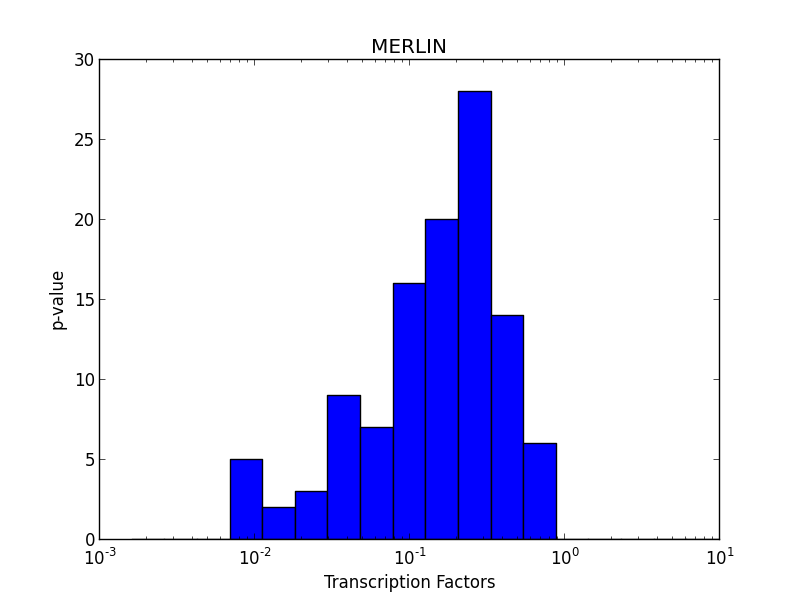
\includegraphics[width=1\linewidth]{./plots/chip_seq_merlin.png}
  \caption{ChIP-seq: MERLIN}
  \label{fig:sub1}
\end{subfigure}%
\begin{subfigure}{.5\textwidth}
  \centering
  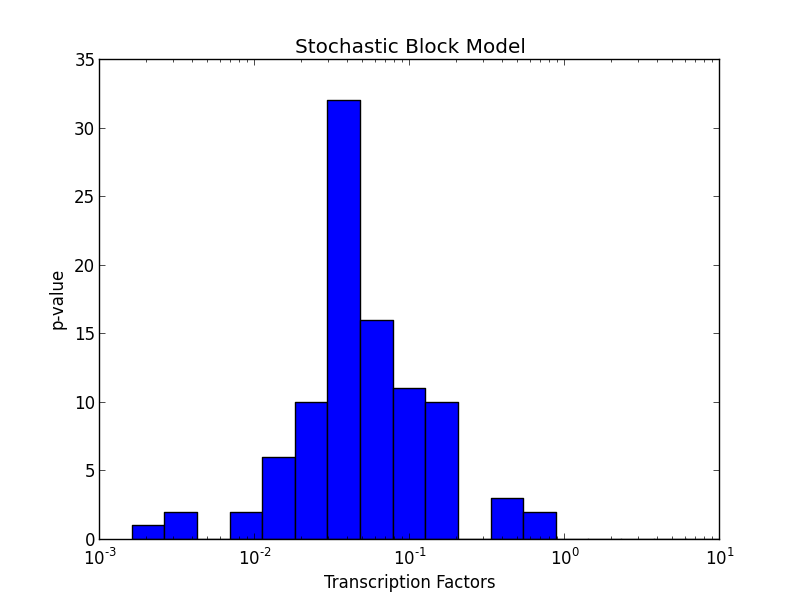
\includegraphics[width=1\linewidth]{./plots/chip_seq_sbm.png}
  \caption{ChIP-seq: Stochastic Block Model}
  \label{fig:sub2}
\end{subfigure}
\caption{The figure shows the p-values of transcription factors for each method}
\label{chipseq}
\end{figure}

To compare results, we have included histograms (for approximately 110 transcription factors) from both MERLIN and our stochastic block model in Figure 1. Note that the average p-value in the Stochastic Block Model is lower than MERLIN, indicating our method outperforms MERLIN. 

\section*{Discussion}

\subsection*{Flexibility of Stochastic Block Model for Clustering}
Using Stochastic Block Model gives a certain flexibility for defining models. Unlike hierarchical clustering, which is rigid and difficult to tune, our model can adapt to user constraints in a number of ways. The input is a binary matrix, which means any method to generate such a binary matrix can be adopted, from simple correlation to more complex models defined by the user. While some may argue that this divides the problem into two parts that may be better suited together, we provide a level of abstraction for generating this binary matrix and clustering. Additionally, our model has learned the transition matrix, priors on cluster assignments, etc. from the data. It is possible to predefine some of these quantities given prior information, allowing for a richer set of models suited to the task at hand. 

\subsection*{Acknowledgements}
We would like to thank Nir Yosef for his support and suggestions on the project, as well as Amelia Wallace, Ling Shen, and Jonathan Kim for their input several parts of the project. We would also like to thank Michael Cole for his discussion and suggestions on estimating the covariance and inverse covariance matrix. 

\subsection*{References}
[1] Vogelstein, B. and Kinzler, K.W. Cancer genes and the pathways they control. Nat Med 10, 789-99 (2004).

[2] Croce, C.M. Oncogenes and cancer. N Engl J Med 358, 502-11 (2008).

[3] Vogelstein, B. et al. Cancer genome landscapes. Science 339, 1546-58 (2013).

[4] Parsons, D.W. et al. An integrated genomic analysis of human glioblastoma multiforme. Science 321, 1807-12 (2008).

[5] Comprehensive genomic characterization defines human glioblastoma genes and core pathways. Nature 455, 1061-8 (2008).

[6] Drier, Y., Sheffer, M. and Domany, E. Pathway-based personalized analysis of cancer. Proc Natl 

Acad Sci U S A 110, 6388-93 (2013).

\end{document}
